% !TeX program = xelatex
% Compile with XeLaTeX (twice) or Tectonic. See README.md for local assets.
\documentclass[aspectratio=169,10pt]{beamer}
\usepackage{fontspec,xeCJK}
\usepackage{tikz,booktabs,tabularx,colortbl}
\usetikzlibrary{arrows.meta,positioning,calc}
\IfFileExists{fonts/NotoSansSC-Regular.ttf}{%
  \setsansfont[Path=fonts/,BoldFont=NotoSansSC-Bold.ttf,ItalicFont=NotoSansSC-Regular.ttf]{NotoSansSC-Regular.ttf}
  \setCJKsansfont[Path=fonts/,BoldFont=NotoSansSC-Bold.ttf,ItalicFont=NotoSansSC-Regular.ttf]{NotoSansSC-Regular.ttf}
  \setCJKmainfont[Path=fonts/,BoldFont=NotoSansSC-Bold.ttf,ItalicFont=NotoSansSC-Regular.ttf]{NotoSansSC-Regular.ttf}
}{%
  \setsansfont[BoldFont=texgyreheros-bold.otf,ItalicFont=texgyreheros-italic.otf]{texgyreheros-regular.otf}
  \setCJKsansfont[BoldFont=FandolHei-Bold.otf]{FandolHei-Regular.otf}
  \setCJKmainfont[BoldFont=FandolHei-Bold.otf]{FandolHei-Regular.otf}
}
\definecolor{Navy}{HTML}{17354C}
\definecolor{Teal}{HTML}{147D80}
\definecolor{Amber}{HTML}{C88722}
\definecolor{Rose}{HTML}{B95B58}
\definecolor{Muted}{HTML}{617783}
\definecolor{Soft}{HTML}{EEF4F6}
\setbeamercolor{normal text}{fg=Navy,bg=white}
\setbeamercolor{frametitle}{fg=Navy,bg=white}
\setbeamercolor{structure}{fg=Teal}
\setbeamercolor{block title}{fg=Navy,bg=Soft}
\setbeamercolor{block body}{fg=Navy,bg=Soft!55}
\setbeamercolor{takeaway}{fg=Navy,bg=Soft}
\setbeamerfont{frametitle}{size=\fontsize{18}{22}\selectfont,series=\bfseries}
\setbeamerfont{block title}{size=\normalsize,series=\bfseries}
\setbeamersize{text margin left=9mm,text margin right=9mm}
\setbeamertemplate{navigation symbols}{}
\setbeamertemplate{itemize items}{\color{Teal}\small\textbullet}
\setbeamertemplate{frametitle}{%
  \vspace{5pt}\usebeamerfont{frametitle}\insertframetitle\par
  \vspace{3pt}{\color{Teal}\rule{18mm}{1.2pt}}\vspace{2pt}}
\setbeamertemplate{footline}{%
  \hspace{9mm}\begin{minipage}{142mm}
  {\color{Muted!35}\hrule}\vspace{3pt}
  {\fontsize{6}{8}\selectfont\color{Muted}eco\_prepro\quad |\quad 实验截至 2026-09-18
  \hfill\insertframenumber\,/\,\inserttotalframenumber}\vspace{4pt}
  \end{minipage}}
\newcommand{\source}[1]{\par\vfill{\fontsize{6.1}{8}\selectfont\color{Muted}#1\par}}
\newcommand{\takeaway}[1]{\vspace{5pt}\begin{beamercolorbox}[wd=\linewidth,sep=6pt]{takeaway}\small #1\end{beamercolorbox}}
\newcommand{\metric}[3]{\begin{minipage}[t]{#1}\centering
  {\fontsize{30}{34}\selectfont\bfseries\color{Teal}#2}\par\vspace{3pt}{\small #3}\end{minipage}}
\newcommand{\panel}[1]{\IfFileExists{assets/#1}{\includegraphics[width=\linewidth]{assets/#1}}{%
  \fbox{\parbox[c][33mm][c]{.96\linewidth}{\centering 本地质检图未打包\par\small 请按 README 复制 assets/\detokenize{#1}}}}}
\newcolumntype{Y}{>{\raggedright\arraybackslash}X}
\setlength{\tabcolsep}{5pt}
\renewcommand{\arraystretch}{1.25}
\hypersetup{pdftitle={心脏超声数据预处理：阶段汇报},pdfauthor={eco-prepro},colorlinks=true,urlcolor=Teal}

\begin{document}

% 01 — outcome first
\begin{frame}[t]
  \vspace{8mm}
  {\small\color{Teal}\bfseries DATA PREPROCESSING / STAGE 1 + STAGE 2}\par\vspace{4mm}
  {\fontsize{26}{32}\selectfont\bfseries 心脏超声数据预处理}\par\vspace{2mm}
  {\fontsize{16}{21}\selectfont 从统一读取到扇形几何优化}\par\vspace{8mm}
  \metric{.31\linewidth}{42}{固定审计条目}\hfill
  \metric{.31\linewidth}{7,318}{累计输入帧}\hfill
  \metric{.31\linewidth}{5}{接受稳定几何拟合}\par\vspace{5mm}
  \takeaway{\textbf{流程与审计已建立；几何有选择地应用。}\quad 整体视觉评级尚未提升。}
  \source{汇报日期：2026-09-25\quad |\quad 实验代码：c2289a9\quad |\quad 基于既有实验记录，未新增数据实验}
\end{frame}

% 02 — data scope
\begin{frame}[t]{42 条目覆盖格式与失败场景}
  \small
  \begin{tabularx}{\linewidth}{@{}l r l Y@{}}
    \rowcolor{Soft}\textbf{来源}&\textbf{数量}&\textbf{格式}&\textbf{验证重点}\\
    EV9V&11&MP4 / JPEG 序列&9 类切面、原始 UI、ECG、暗区、长视频\\
    EchoNet-Dynamic&3&AVI&已预处理输入直接保留\\
    EchoNet-Pediatric&4&AVI&儿科输入及已有边缘标记\\
    EchoNet-LVH&6&AVI&大尺寸输入、帧率来源差异\\
    CAMUS&7&NIfTI / MHD&医学图像读取与时序信息\\
    Unity&6&PNG&静态界面、暗区、染色 B-mode\\
    DICOM 测试样本&5&DICOM&4 个非心脏静态样本＋1 个历史彩色 cine\\
    \bottomrule
  \end{tabularx}
  \vspace{4pt}
  \begin{itemize}\setlength{\itemsep}{2pt}
    \item \textbf{工程审计条目不等于独立患者。}JPEG 与 MHD 含已有来源的衍生输入。
    \item 最长视频 \textbf{3,243 帧}；7,318 帧为全部条目之和，包含衍生条目。
    \item 现代彩色 Doppler、原始 GE 动态视频、多厂商泛化尚未覆盖。
  \end{itemize}
  \source{依据：configs/audit\_manifest.csv；docs/audit\_results\_stage2.csv}
\end{frame}

% 03 — frozen infrastructure
\begin{frame}[t]{Stage 1：统一输入与可追溯处理}
  \begin{center}
  \begin{tikzpicture}[node distance=3mm and 4mm,>=Stealth,
    flow/.style={draw=Teal!35,fill=Soft,rounded corners=2pt,minimum height=12mm,text width=22mm,align=center,font=\small}]
    \node[flow] (a) {异构输入\\视频 / 图像};
    \node[flow,right=of a] (b) {Cine\\帧序列＋元数据};
    \node[flow,right=of b] (c) {状态分流\\质量控制};
    \node[flow,right=of c] (d) {裁剪或保留\\全部帧输出};
    \node[flow,right=of d] (e) {视频＋JSON\\质检图＋审计表};
    \foreach \u/\v in {a/b,b/c,c/d,d/e}\draw[->,Teal,thick] (\u)--(\v);
  \end{tikzpicture}
  \end{center}
  \vspace{3pt}
  \begin{columns}[T,onlytextwidth]
  \column{.31\textwidth}
    \begin{block}{已预处理输入}\small PASSTHROUGH\\直接保留像素与画布\end{block}
  \column{.31\textwidth}
    \begin{block}{可信动态输入}\small SUCCESS\\裁剪、掩膜、方形补边\end{block}
  \column{.34\textwidth}
    \begin{block}{不确定或特殊输入}\small 低置信度 / 静态 / 多区域\\保留原图，记录复核原因\end{block}
  \end{columns}
  \vspace{3pt}\small
  \begin{itemize}\setlength{\itemsep}{3pt}
    \item SHA-256 固定案例身份；分别保存容器帧率、数据表帧率和采用来源。
    \item 最多 64 个采样帧计算时间标准差＋亮度支持；处理与导出使用全部帧。
    \item Stage 2 保持读取、Cine、溯源、导出和审计基础设施冻结。
  \end{itemize}
  \source{依据：docs/STAGE1.md；docs/stage2\_frozen\_contract.json}
\end{frame}

% 04 — geometry method with native vector schematics
\begin{frame}[t]{Stage 2：运动找位置，几何恢复形状}
  \begin{center}
  \begin{tikzpicture}[>=Stealth,box/.style={draw=Teal!40,fill=Soft,rounded corners=2pt,
      minimum height=11mm,text width=28mm,align=center,font=\small}]
    \node[box] (a) at (0,0) {allowed area\\内的运动与支持区域};
    \node[box] (b) at (3.5,0) {多种几何拟合\\掩膜限制在允许区域};
    \node[box] (c) at (7,0) {证据可靠性\\残差、覆盖、切入深度};
    \node[box] (d) at (10.5,0) {时间稳定性\\不同采样保持一致};
    \foreach \u/\v in {a/b,b/c,c/d}\draw[->,Teal,thick] (\u)--(\v);
  \end{tikzpicture}
  \end{center}
  \vspace{2pt}
  \begin{center}
  \begin{tikzpicture}[scale=.78,sectorstyle/.style={fill=Teal!13,draw=Teal,line width=.9pt}]
    \draw[sectorstyle] (0,0)--(225:1.05) arc[start angle=225,end angle=315,radius=1.05]--cycle;
    \node[font=\small] at (0,-1.5) {标准扇形};
    \begin{scope}[shift={(4.2,0)}]
      \draw[sectorstyle] (-.22,-.22)--(225:1.05) arc[start angle=225,end angle=315,radius=1.05]--(.22,-.22)--cycle;
      \node[font=\small] at (0,-1.5) {平顶 / 虚拟顶点};
    \end{scope}
    \begin{scope}[shift={(8.4,0)}]
      \begin{scope}[rotate=30]\draw[sectorstyle] (0,0)--(240:1.05) arc[start angle=240,end angle=300,radius=1.05]--cycle;\end{scope}
      \node[font=\small] at (0,-1.5) {旋转楔形};
    \end{scope}
    \begin{scope}[shift={(12.6,0)}]
      \draw[sectorstyle] (-.65,-.95) rectangle (.65,-.1);
      \node[font=\small] at (0,-1.5) {矩形};
    \end{scope}
  \end{tikzpicture}
  \end{center}
  \small
  \textbf{布局排除：}已验证 EV9V 的顶部文字、灰条、外侧刻度及 ECG 区域。\\[3pt]
  \textbf{接受条件：}跨采样掩膜两两 IoU $\geq 0.98$；与最终候选 IoU $\geq 0.97$。\\[3pt]
  \textbf{拒绝后：}复用原先可信的凸包；原始证据不足则保留整幅图像。
  \takeaway{每段视频使用一个固定掩膜；不生成图像内容，不预设固定扇形模板。}
  \source{形状为示意。平顶、旋转单区域和矩形动态心超目前仅有合成验证。依据：sector/geometry.py、motion.py。}
\end{frame}

% 05 — experiment protocol
\begin{frame}[t]{实验：固定子集定稿，再做全量回归}
  \begin{center}
  \begin{tikzpicture}[>=Stealth]
    \node[fill=Soft,rounded corners=2pt,align=center,text width=38mm,minimum height=13mm] (a) at (0,0) {\textbf{10 条目子集}\\\small 7 个动态＋3 个保留对照};
    \node[fill=Soft,rounded corners=2pt,align=center,text width=23mm,minimum height=13mm] (b) at (4.4,0) {\textbf{冻结阈值}\\\small 不再调参};
    \node[fill=Soft,rounded corners=2pt,align=center,text width=38mm,minimum height=13mm] (c) at (8.8,0) {\textbf{42 条目全量}\\\small 包含上述 10 条目};
    \draw[->,Teal,thick] (a)--(b);\draw[->,Teal,thick] (b)--(c);
  \end{tikzpicture}
  \end{center}
  \small
  \begin{tabularx}{\linewidth}{@{}l Y l@{}}
    \rowcolor{Soft}\textbf{验证项目}&\textbf{实验设置}&\textbf{结果}\\
    读取与导出&全帧解码；核对尺寸、帧数、帧率&42/42 通过\\
    Stage 1 兼容&与 b494f9f 的 mask、状态和统计逐条比较&42/42 一致\\
    像素保留&直接保留＋待复核分支的内存输出&33/33 一致\\
    合成几何&已知真值；多形状、暗缺口、排除区域&扇形 IoU $>0.96$\\
    时间稳定性&改变采样密度及奇偶采样相位&不稳定拟合被拒绝\\
    工程检查&保留策略、拒绝机制、接口与冻结文件&46 项测试通过\\
    \bottomrule
  \end{tabularx}
  \takeaway{全量审计包含调试子集，\textbf{不是独立测试集}；合成真值结果不替代真实分割准确率。}
  \source{依据：tests/test\_stage2.py；docs/stage2\_verification.json；docs/audit\_export\_verification\_stage2.csv。MP4 编码为有损。}
\end{frame}

% 06 — status is not visual quality
\begin{frame}[t]{42 个输出完成验证，处理状态未变}
  \begin{columns}[T,onlytextwidth]
  \column{.53\textwidth}
    \small
    \begin{tabularx}{\linewidth}{@{}Y r r@{}}
      \rowcolor{Soft}\textbf{状态}&\textbf{Stage 1}&\textbf{Stage 2}\\
      SUCCESS&9&9\\
      PASSTHROUGH&20&20\\
      LOW\_CONFIDENCE&2&2\\
      STATIC&9&9\\
      MULTI\_REGION&2&2\\
      FAILED&0&0\\
      \bottomrule
    \end{tabularx}
  \column{.43\textwidth}
    \begin{block}{11 个 EV9V 动态条目}
      \small\textbf{5} 个接受标准扇形拟合\\[4pt]
      \textbf{4} 个使用可信凸包\\[4pt]
      \textbf{2} 个保留原图
    \end{block}
    \small 其余 \textbf{31} 个直接保留、静态和多区域条目，跳过几何拟合。
  \end{columns}
  \vspace{4pt}\small
  \textbf{最长视频 3,243 帧完整导出。}全部 42 个视频可完整解码，运行失败数为 0。
  \takeaway{SUCCESS 表示执行了裁剪流程；\textbf{不等于视觉质检 PASS}。}
  \source{依据：docs/audit\_results\_stage1.csv、audit\_results\_stage2.csv。MULTI\_REGION 含一个未修正的 Unity 静帧误判。}
\end{frame}

% 07 — quantitative fit outcomes
\begin{frame}[t]{5 个接受拟合条目的时间稳定性}
  \small\renewcommand{\arraystretch}{1.10}
  \begin{tabularx}{\linewidth}{@{}Y c r r@{}}
    \rowcolor{Soft}\textbf{条目}&\textbf{调试子集}&\textbf{最低采样 IoU}&\textbf{证据保留率}\\
    A4C&是&0.9943&99.73\%\\
    PLHLA&否&0.9951&99.76\%\\
    PMPALA&否&0.9937&99.60\%\\
    PPMLSA&是&0.9958&99.77\%\\
    3,243 帧长视频&否&0.9927&99.66\%\\
    \bottomrule
  \end{tabularx}
  \vspace{5pt}
  \begin{columns}[T,onlytextwidth]
  \column{.47\textwidth}
    \begin{block}{边界恢复的幅度}\small 相对候选区域，拟合掩膜面积增加\par\vspace{4pt}
    {\Large\bfseries\color{Teal}3.2\%--5.8\%}\end{block}
  \column{.49\textwidth}
    \begin{block}{指标的含义}\small IoU：不同时间采样之间的一致性。\\[4pt]
    保留率：对算法候选区域的覆盖。\end{block}
  \end{columns}
  \takeaway{尚无人工 sector mask；面积补全、稳定性和候选覆盖\textbf{均不等于真实解剖保留率}。}
  \source{依据：docs/audit\_results\_stage2.csv；几何通过并不代表已清除所有 UI 标记。}
\end{frame}

% 08 — actual release example, private local asset
\begin{frame}[t]{实际案例：A4C 接受稳定扇形拟合}
  \panel{normal_fan.png}
  \vspace{2pt}
  \begin{columns}[T,onlytextwidth]
    \column{.30\textwidth}\small\textbf{最低采样 IoU}\\{\Large\color{Teal}0.9943}
    \column{.30\textwidth}\small\textbf{候选证据保留}\\{\Large\color{Teal}99.73\%}
    \column{.35\textwidth}\small\textbf{剩余问题}\\边缘刻度及部分 ECG 尖峰仍可能残留。
  \end{columns}
  \source{本地 Stage 2 四联图：ev9v\_d47d8e7414433eb2。EV9V：Bo Gou 等，CC BY 4.0；本项目生成处理及标注面板。}
\end{frame}

% 09 — abstention is a result, not a geometry success
\begin{frame}[t]{实际案例：PASA 暗区仍保留原图}
  \panel{dark_sector.png}
  \vspace{1pt}\small
  \textbf{原因：}侧边与外弧证据不足，不能可靠推断完整扇形。\\[4pt]
  \textbf{其他拒绝案例：}PMASA 的采样 IoU 0.9540，回退凸包；JPEG 为 0.8022，保留原图。
  \source{本地 Stage 2 四联图：ev9v\_a9b7d8c2e96c23f1。EV9V：Bo Gou 等，CC BY 4.0；合成暗缺口恢复不代表该真实暗区已解决。}
\end{frame}

% 10 — visual readiness must be separated from successful execution
\begin{frame}[t]{视觉质检：整体评级尚未提升}
  \begin{center}
  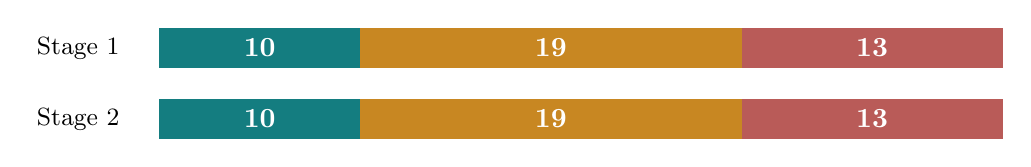
\begin{tikzpicture}[x=.255cm,y=.9cm]
    \foreach \yy/\label in {1/Stage 1,0/Stage 2}{
      \node[anchor=east,font=\small] at (-1.5,\yy+.28) {\label};
      \fill[Teal] (0,\yy) rectangle (10,\yy+.57);
      \fill[Amber] (10,\yy) rectangle (29,\yy+.57);
      \fill[Rose] (29,\yy) rectangle (42,\yy+.57);
      \node[text=white,font=\bfseries] at (5,\yy+.285) {10};
      \node[text=white,font=\bfseries] at (19.5,\yy+.285) {19};
      \node[text=white,font=\bfseries] at (35.5,\yy+.285) {13};
    }
  \end{tikzpicture}\par\vspace{4pt}
  {\small\color{Teal}PASS}\quad
  {\small\color{Amber}MINOR\_ISSUE}\quad
  {\small\color{Rose}FAIL}
  \end{center}
  \small
  \begin{itemize}\setlength{\itemsep}{5pt}
    \item \textbf{19 个轻微问题：}边缘刻度、细线、ECG 尖峰及输入自带标记。
    \item \textbf{13 个 FAIL：}正确保留的未解决原始输入，不是程序运行失败。
    \item 评级来自助手对比图及导出首／中／末帧检查；独立人工复核仍未完成。
  \end{itemize}
  \takeaway{本阶段证明流程可追溯、拟合可拒绝；\textbf{尚未证明整体图像清理质量提升}。}
  \source{依据：docs/audit\_visual\_review\_stage1.csv、audit\_visual\_review\_stage2.csv。柱形单位为审计条目。}
\end{frame}

% 11 — direct close, no generic thank-you slide
\begin{frame}[t]{结论与下一步}
  \begin{columns}[T,onlytextwidth]
  \column{.48\textwidth}
    \begin{block}{已完成}\small
      \begin{itemize}\setlength{\itemsep}{5pt}
        \item 统一读取、帧率与元数据溯源。
        \item 固定审计、全帧导出和保留策略。
        \item 首版几何拟合＋时间稳定性拒绝。
        \item 42 个导出验证；46 项测试通过。
      \end{itemize}
    \end{block}
  \column{.48\textwidth}
    \begin{block}{待验证／待解决}\small
      \begin{itemize}\setlength{\itemsep}{5pt}
        \item 真实暗区与边界标记残留。
        \item 静态、多区域、现代彩色 Doppler。
        \item 平顶／旋转／矩形的真实动态样本。
        \item 独立人工真值及跨厂商泛化。
      \end{itemize}
    \end{block}
  \end{columns}
  \vspace{5pt}
  \takeaway{\textbf{下一步：}固定案例补充人工评级和 sector mask，量化边界误差、解剖裁切与 UI 残留；单区域动态 cine 稳定后，再决定 Stage 3。}
  \source{数据与结果：仓库 configs/、docs/ 下的冻结清单与审计表。\\
    \href{https://github.com/yuanshu777/eco_prepro}{github.com/yuanshu777/eco\_prepro}\quad |\quad 本次仅汇报已有实验；图像与完整演示包保留本地。}
\end{frame}

\end{document}
